\documentclass[9pt]{beamer}

\usefonttheme{serif}
\usepackage{ebgaramond}

\usepackage[utf8]{inputenc}
\usepackage[english]{babel}
\usepackage{minted}
\usepackage{graphicx}
\usepackage{hyperref}
\usepackage{ amssymb }
\usepackage{ multirow }
\usepackage{ csquotes }

\usemintedstyle{vs}

\setbeamertemplate{navigation symbols}{}
\setbeamertemplate{footline}[frame number]{}

\renewcommand\big[1]{
  \begin{center}
    \Large{#1}
  \end{center}
}

\newcounter{ruleCounter}

\newcommand\ruleNum[0]{\stepcounter{ruleCounter}\arabic{ruleCounter}}


\begin{document}

\begin{frame}[plain]
  \centering\Huge{Introduction to Memory Management in Rust}
\end{frame}

\begin{frame}
  \big{1. Explain how Rust ended up with its memory system}

  \big{2. Give a high-level picture of how memory works in Rust}
\end{frame}

\begin{frame}
  \centering\Huge{The (Shortened and Possibly Inaccurate) Story of Memory Management in Rust}
\end{frame}

\begin{frame}
  \big{Motivation for Rust: build a fast, parallel, and safe browser engine.}

  \begin{itemize}
    \item Browsers did not exploit the machines' parallelism (image decoding, CSS layout)
    \item Browsers had\footnote{They still do.} security flaws that were exploitable (Pwn2Own)
  \end{itemize}
\end{frame}

\begin{frame}
  \big{The original author, Graydon Hoare, envisioned Rust to be:}

  \begin{itemize}
    \item Fast: run on the metal, not in a VM;
    \item Parallel: easy(ier) to write correct parallel code;
    \item Type safe: operations on objects are always compatible with the object's type;
    \item Memory safe: no incorrect usage of memory at run-time.
  \end{itemize}
\end{frame}

\begin{frame}
  \big{Early Rust was quite a different language from today:}

  \begin{itemize}
    \item Written in OCaml;
    \item ML-inspired syntax;
    \item Iterators were a special construct;
    \item Type-state system\footnote{Original idea for Rust, abandonned because it was too much of a chore to use in practice};
    \item Automatic memory management via garbage collection.
  \end{itemize}
\end{frame}

\begin{frame}
  \big{Garbage collection turned out to be an issue:}
  \begin{itemize}
    \item It offers memory safety, but:
    \item Running garbage collection takes precious time;
    \item Extra boxing + fields for GC are not cache-friendly.
  \end{itemize}
\end{frame}

\begin{frame}
  \big{Problem}
  \begin{itemize}
    \item Retain memory safety (i.e., automatic memory management);
    \item Don't pay for that safety at run-time.
  \end{itemize}
\end{frame}

\begin{frame}
  \big{Solution}
  \begin{itemize}
    \item Insert \emph{free()} calls at compile-time;
    \item The compiler must understand memory usage;
    \item Restrict how pointers can be used;
    \item Reject code that would be fine at execution.
  \end{itemize}
\end{frame}

\begin{frame}
  \textquote[Programming~Rust, O'Reilly]{
    \sl Rust's radical wager---the claim on which it stakes its success, and
    that forms the root of the language---is that even with these
    restrictions in place, you'll find the language more than flexible
    enough for almost every task, and that the benefits---the elimination
    of broad classes of memory management and concurrency bugs—will
    justify the adaptations you'll need to make to your style. The authors
    of this book are bullish on Rust exactly because of our extensive
    experience with C and C++. For us, Rust's deal is a no-brainer.
  }
\end{frame}


\begin{frame}
  \centering\Huge{How to Manage Memory in Rust}
\end{frame}

\begin{frame}
  \big{\ruleNum. An object has a \emph{single} owner}

  \big{\ruleNum. An object is dropped when its owner goes out of scope}
\end{frame}

\begin{frame}[fragile]
  \inputminted{rust}{demos/00_dealloc.rs}
\end{frame}

\begin{frame}
  \big{\ruleNum. An assignment makes a \emph{shallow copy} and \emph{transfers ownership}}

  \big{\ruleNum. A variable that owns no object cannot be used}
\end{frame}

\begin{frame}[fragile]
  \inputminted{rust}{demos/01_move.rs}

  \footnotesize{Example of program that would work, but is rejected.}
\end{frame}

\begin{frame}[fragile]
  \inputminted{rust}{demos/03_func_move.rs}
\end{frame}

\begin{frame}[fragile]
  \inputminted{rust}{demos/04_retransfer.rs}
\end{frame}

\begin{frame}
  \big{\ruleNum. Some object types do a \emph{full copy} rather than transfer ownership}
\end{frame}

\begin{frame}[fragile]
  \inputminted{rust}{demos/02_copy.rs}
\end{frame}

\begin{frame}
  \big{\ruleNum. A \emph{shared borrow} is a read-only pointer to an object}

  \big{\ruleNum. A borrow does not own the object it points to}
\end{frame}

\begin{frame}[fragile]
  \inputminted{rust}{demos/05_borrow.rs}
\end{frame}

\begin{frame}
  \big{\ruleNum. Many shared borrows to the same object are allowed}
\end{frame}

\begin{frame}[fragile]
  \inputminted{rust}{demos/06_multiple_shared_borrows.rs}
\end{frame}

\begin{frame}
  \big{\ruleNum. A \emph{mutable borrow} is a read-write pointer to an object}
\end{frame}

\begin{frame}[fragile]
  \inputminted{rust}{demos/07_mut_borrow.rs}
\end{frame}

\begin{frame}
  \big{\ruleNum. A single mutable borrow to an object may exist at any given time}
\end{frame}

\begin{frame}[fragile]
  \inputminted{rust}{demos/08_single_mut_borrow.rs}
\end{frame}

\begin{frame}
  \big{\ruleNum. Shared and mutable borrows to the same object cannot coexist}
\end{frame}

\begin{frame}[fragile]
  \inputminted{rust}{demos/09_mutex_borrows.rs}
\end{frame}

\begin{frame}
  \centering\Huge{Interlude}

  \big{Why can't shared and mutable borrows coexist?}
\end{frame}

\begin{frame}[fragile]
  \inputminted{c++}{demos/interlude.cpp}
\end{frame}

\begin{frame}
  \centering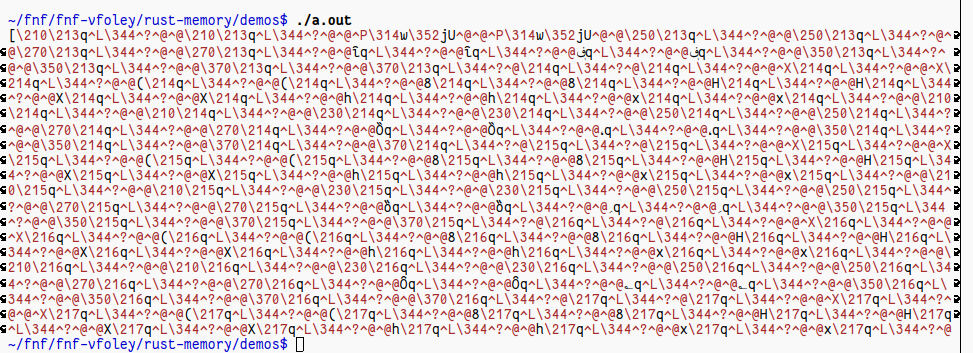
\includegraphics[scale=0.32]{demos/boom.png}
\end{frame}

\begin{frame}
  \big{Mixing \emph{aliasing} and \emph{mutablility} is often problematic}

  \big{Rust disallows it}

  \centering\Huge{/Interlude}
\end{frame}

\begin{frame}
  \big{\ruleNum. A borrow must finish before the owner goes out of scope}
\end{frame}

\begin{frame}[fragile]
  \inputminted{rust}{demos/10_too_long.rs}
\end{frame}

\begin{frame}
  \big{\ruleNum. Only the owner can transfer ownership of its object and only when there are no borrows}
\end{frame}

\begin{frame}[fragile]
  \inputminted{rust}{demos/11_move_out.rs}
\end{frame}

\begin{frame}[fragile]
  \inputminted{rust}{demos/12_move_out.rs}
\end{frame}

\begin{frame}
  \centering\Huge{Interlude}

  \big{Moving out of vectors and structs}
\end{frame}

\begin{frame}[fragile]
  \big{An object \emph{cannot} be moved out of a vector element:}
\end{frame}

\begin{frame}[fragile]
  \inputminted{rust}{demos/13_move_out_vec.rs}
\end{frame}

\begin{frame}[fragile]
  \big{An object \emph{can} be moved out of a struct field:}
\end{frame}

\begin{frame}[fragile]
  \inputminted{rust}{demos/14_move_out_struct.rs}
\end{frame}

\begin{frame}
  \centering\Huge{/Interlude}
\end{frame}

\end{document}
